% Template for ICASSP-2010 paper; to be used with:
%          mlspconf.sty  - ICASSP/ICIP LaTeX style file adapted for MLSP, and
%          IEEEbib.bst - IEEE bibliography style file.
% --------------------------------------------------------------------------
\documentclass{article}
\usepackage{amsmath,graphicx,02460}

%%%%%%%%%%%%%%%%%%%%%%%%%%%%%%%%%%%%%%%%%%%%%%%%%%%%%%%%%%%%%%%%%%%%%%%%%%%%%%
% Zach added packages
\usepackage{todonotes}
\usepackage{acronym}
\newacro{HI}{Hello World!}
\newacro{ASR}{Automatic Speech Recognition}
\newacro{STOI}{Short Time Objective Intelligibility Measure}
\newacro{PESQ}{Perceptual Evaluation of Speech Quality}

\graphicspath{{figures/}}
\usepackage{subcaption}
\usepackage{booktabs}
\usepackage{hyperref}
\hypersetup{
	colorlinks=true,
	linkcolor=black,
	urlcolor=black,
	citecolor=black,
}
%%%%%%%%%%%%%%%%%%%%%%%%%%%%%%%%%%%%%%%%%%%%%%%%%%%%%%%%%%%%%%%%%%%%%%%%%%%%%%


\toappear{02456 Deep Learning, DTU Compute, Fall 2019}


% Example definitions.
% --------------------
\def\x{{\mathbf x}}
\def\L{{\cal L}}

% Title.
% ------
\title{Speech Dereverberation with U-Net Architectures}
%
% Single address.
% ---------------
\name{Zachary Neveu}
\address{Technical University of Denmark}
	
%
% For example:
% ------------
%\address{School\\
%	Department\\
%	Address}
%
% Two addresses (uncomment and modify for two-address case).
% ----------------------------------------------------------
%\twoauthors
%  {A. Author-one, B. Author-two\sthanks{Thanks to XYZ agency for funding.}}
%	{School A-B\\
%	Department A-B\\
%	Address A-B}
%  {C. Author-three, D. Author-four\sthanks{The fourth author performed the work
%	while at ...}}
%	{School C-D\\
%	Department C-D\\
%	Address C-D}
%
\begin{document}
%\ninept
%

\maketitle
%

\begin{center}
\raisebox{-3pt}{
\includegraphics[height=11pt]{figures/github.png}}\ \ \href{https://github.com/zacharyneveu/DeReverb}{\texttt{github.com/zacharyneveu/DeReverb}}
\end{center}

\begin{abstract}
This work compares the performance of time and frequency domain approaches to speech dereverberation using u-net architectures. Towards this end, a neural architecture is constructed consisting of a u-net with a recurrent latent layer. Two models of this architecture are trained, one using time-domain inputs, one using frequency domain magnitudes. Results are compared using the \ac{STOI} and \ac{PESQ} metrics. Additionally, a simple frequency-domain perceptually weighted loss function is presented.

\end{abstract}
%
\begin{keywords}
Speech, Enhancement, Reverb, Noise
\end{keywords}
%
\section{Introduction}
\label{sec:intro}
\small{In real world environments, speech is heard as a mix of direct signal with reflections caused by the surrounding environment. Late reflections decrease speech intelligibility, causing problems for listeners, as well as tasks such as \ac{ASR} \todo[inline]{cite}. Using multiple microphones, reverberation can be removed by exploiting the spatial differences between direct and reverberant sound, however this requires increased hardware cost. An algorithm is then required which can remove the effects of reverberation using only a single channel of audio. Traditional signal processing approaches can solve this problem, however these algorithms typically do not leverage the structure of speech, as this is difficult to model mathematically. Neural networks have the capability to learn the structure of speech from data, potentially allowing for superior performance to traditional algorithms.}


\section{Model Architecture}%
\label{sec:model_architecture}
\begin{figure}[h]
\begin{center}
	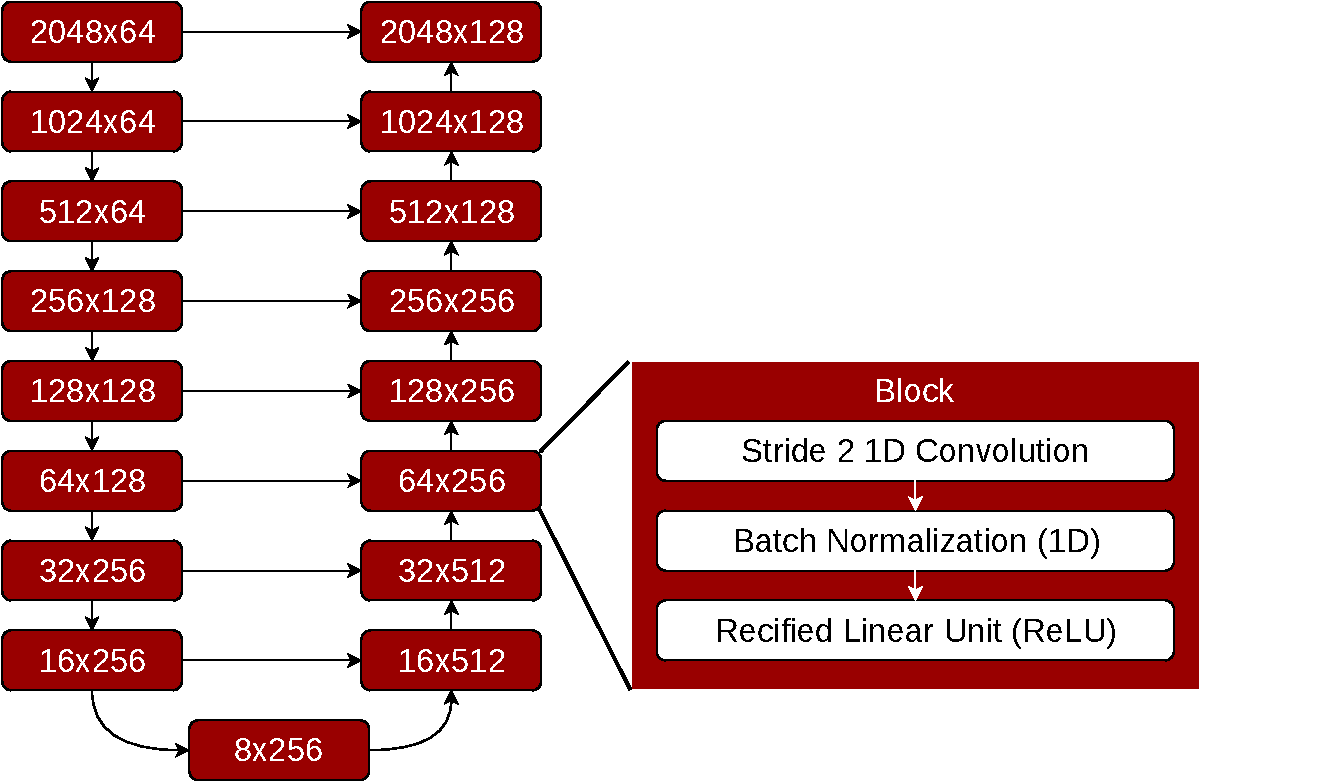
\includegraphics[width=0.5\textwidth]{architecture}
	\caption{Model Architecture}
	\label{fig:architecture}
\end{center}
\end{figure}

\noindent Two networks are trained which are both based on the u-net architecture originally proposed in \cite{ronneberger_u-net_2015} and used for speech enhancement/denoising in \cite{pandey_new_2019}.  The reasoning behind using a u-net architecture is that speech is known to be sparse, and can be represented well with a small amount of data. The information bottleneck of a u-net architecture should allow the network to distill salient information about the speech, while the pass-through connections allow for the recreation of utterance-specific details. Additionally, the 1-dimensional convolution layers used are known to be useful for frequency analysis, enabling the time-domain network to learn frequency-domain features. The specific layer sizes and the architecture of each block is detailed in figure \ref{fig:architecture}. A \ac{LSTM} layer is used to filter the latent representation of the speech stored in the bottleneck of the u-net. This architecture modification is used in \cite{defossez_music_nodate} for source separation and is based on the intuition that each frame of sound processed is highly dependent on past frames. The time-domain network replaces the final rectified linear unit activation with a hyperbolic tangent activation to produce values between -1 and 1. The frequency domain network is one block in a larger traditional signal processing system shown in figure \ref{fig:systems}.

\begin{figure}[h]
	\centering
	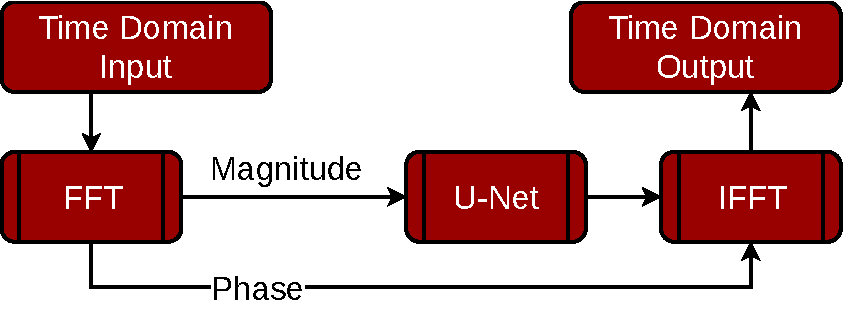
\includegraphics[width=0.5\textwidth]{systems_2}
	\caption{System Architecture of Frequency domain Network}
	\label{fig:systems}
\end{figure}


\section{Data}%
\label{sec:data}
The training data consists of a subset of the LibriSpeech dataset \cite{panayotov_librispeech_2015} which is processed according to the pipeline shown in figure \ref{fig:data_pipeline}. In total, the dataset consists of 2255 speech utterances, 36 impulse responses, and 20 noise recordings. In order to avoid overfitting, each time a speech file is loaded, it is randomly cropped, then paired with a segment of a randomly chosen noise file and a randomly chosen impulse response. In the data pipeline presented, noise is added before the convolution takes place. This is done in an effort to model real rooms where ambient noises are also convolved with the reverberation of the room. This ordering is important to note, as most approaches use the reverse ordering.	It is also important to note that the result of the convolution operation is truncated to retain the same length as the target signal. This is necessary so that the loss function can be easily be computed between the network output and the target.

\begin{figure}[h]
	\centering
	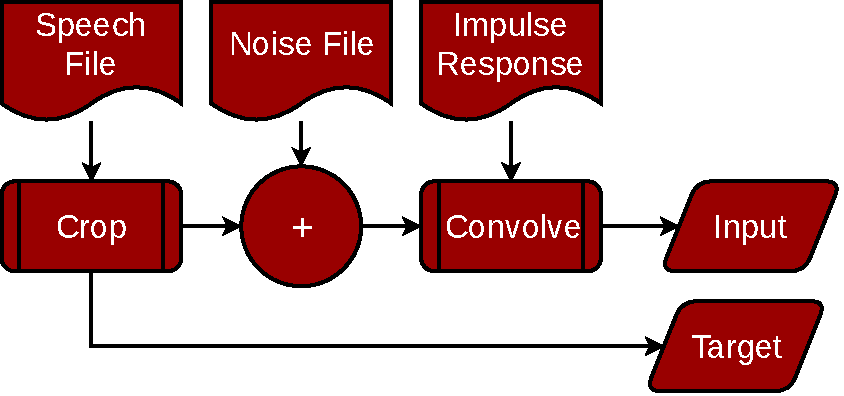
\includegraphics[width=0.5\textwidth]{data_pipeline}
	\caption{Data pipeline}
	\label{fig:data_pipeline}
\end{figure}


\section{Training}%
\label{sec:data_and_training}
The training data consists of a subset of the LibriSpeech dataset \cite{panayotov_librispeech_2015} which is processed according to the pipeline shown in figure \ref{fig:data_pipeline}. Both models are trained on this data for 15 epochs using the Adam optimizer. Training is stopped at this point because losses have largely stopped decreasing and training is slow because of large file sizes of inputs.

\begin{figure}[h]
	\centering
	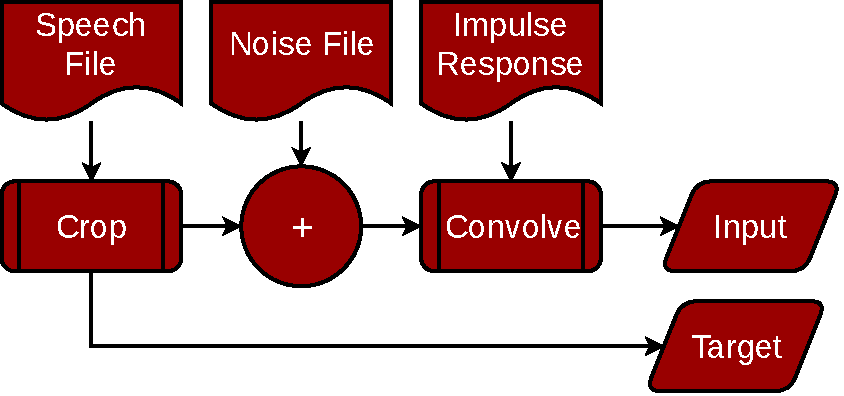
\includegraphics[width=0.5\textwidth]{data_pipeline}
	\caption{Data pipeline}
	\label{fig:data_pipeline}
\end{figure}


\section{Results}%
\label{sec:results}
\begin{figure}
	\centering
	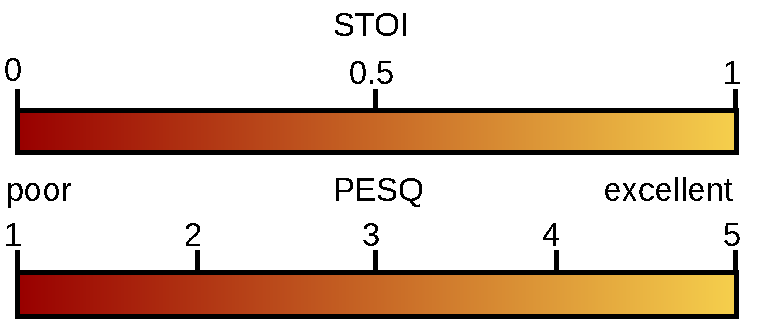
\includegraphics[width=0.5\textwidth]{metrics}
	\caption{\ac{PESQ} and \ac{STOI} metric scales}
	\label{fig:metrics}
\end{figure}

\begin{table}
	\centering
	\caption{mean change STOI and PESQ scores for a subset of the validation set}
	\label{tab:results}
	\resizebox{0.5\textwidth}{!} {
	\begin{tabular}{lrr}
	\toprule
			  Method &  avg. $\Delta$STOI &  \ avg. $\Delta$PESQ \\
	\midrule
	Frequency-domain &         0.070 &        -0.383 \\
		 Time-domain &         0.023 &        -0.159 \\
	\bottomrule
	\end{tabular}
	}
\end{table}

To evaluate the results, two common speech metrics are used: \ac{STOI} and \ac{PESQ}. \ac{STOI} measures speech intelligibility, whereas \ac{PESQ} measures speech quality. Figure \ref{fig:metrics} shows the scaling for each score. Both \ac{PESQ} and \ac{STOI} are intended to be used on segments of speech that are many frames long. In order to measure results in this manner, a long segment of speech is reconstructed using the \ac{WOLA} method \todo[inline]{cite if i can find this...}. This method was chosen over concatenating adjacent frames because it lessens the severity of discontinuities at frame boundaries. The \ac{WOLA} method consists of reconstructing frames that overlap by a constant number of samples. Reconstructed frames are multiplied by a Hann window. All frames are then added together with respective offsets to create the final reconstructed signal. Table \ref{tab:results} shows the mean change in the speech metric scores for 10 reconstructed random  examples from the validation set. Both the time-domain and frequency-domain networks improve the \ac{STOI} while making the \ac{PESQ} worse. These networks may be useful for tasks such as \ac{ASR} where intelligibility is valued over quality. Notably, the frequency-domain network achieved both a larger boost in \ac{STOI} and a larger detriment to the \ac{PESQ} than the time-domain network. Figure \ref{fig:specs} shows spectrograms for the input, target, and both models for an example speech sequence.

\begin{figure}
	\centering
	\includegraphics[width=0.5\textwidth]{../../project/figs/specs2}
	\caption{Spectrograms of Reconstructed Example}
	\label{fig:specs}
\end{figure}




% References should be produced using the bibtex program from suitable
% BiBTeX files (here: strings, refs, manuals). The IEEEbib.bst bibliography
% style file from IEEE produces unsorted bibliography list.
% -------------------------------------------------------------------------
\bibliographystyle{IEEEbib}
\bibliography{refs}

\end{document}
